\documentclass[letterpaper,12pt]{article}\usepackage[]{graphicx}\usepackage[]{color}
%% maxwidth is the original width if it is less than linewidth
%% otherwise use linewidth (to make sure the graphics do not exceed the margin)
\makeatletter
\def\maxwidth{ %
  \ifdim\Gin@nat@width>\linewidth
    \linewidth
  \else
    \Gin@nat@width
  \fi
}
\makeatother

\definecolor{fgcolor}{rgb}{0.345, 0.345, 0.345}
\newcommand{\hlnum}[1]{\textcolor[rgb]{0.686,0.059,0.569}{#1}}%
\newcommand{\hlstr}[1]{\textcolor[rgb]{0.192,0.494,0.8}{#1}}%
\newcommand{\hlcom}[1]{\textcolor[rgb]{0.678,0.584,0.686}{\textit{#1}}}%
\newcommand{\hlopt}[1]{\textcolor[rgb]{0,0,0}{#1}}%
\newcommand{\hlstd}[1]{\textcolor[rgb]{0.345,0.345,0.345}{#1}}%
\newcommand{\hlkwa}[1]{\textcolor[rgb]{0.161,0.373,0.58}{\textbf{#1}}}%
\newcommand{\hlkwb}[1]{\textcolor[rgb]{0.69,0.353,0.396}{#1}}%
\newcommand{\hlkwc}[1]{\textcolor[rgb]{0.333,0.667,0.333}{#1}}%
\newcommand{\hlkwd}[1]{\textcolor[rgb]{0.737,0.353,0.396}{\textbf{#1}}}%
\let\hlipl\hlkwb

\usepackage{framed}
\makeatletter
\newenvironment{kframe}{%
 \def\at@end@of@kframe{}%
 \ifinner\ifhmode%
  \def\at@end@of@kframe{\end{minipage}}%
  \begin{minipage}{\columnwidth}%
 \fi\fi%
 \def\FrameCommand##1{\hskip\@totalleftmargin \hskip-\fboxsep
 \colorbox{shadecolor}{##1}\hskip-\fboxsep
     % There is no \\@totalrightmargin, so:
     \hskip-\linewidth \hskip-\@totalleftmargin \hskip\columnwidth}%
 \MakeFramed {\advance\hsize-\width
   \@totalleftmargin\z@ \linewidth\hsize
   \@setminipage}}%
 {\par\unskip\endMakeFramed%
 \at@end@of@kframe}
\makeatother

\definecolor{shadecolor}{rgb}{.97, .97, .97}
\definecolor{messagecolor}{rgb}{0, 0, 0}
\definecolor{warningcolor}{rgb}{1, 0, 1}
\definecolor{errorcolor}{rgb}{1, 0, 0}
\newenvironment{knitrout}{}{} % an empty environment to be redefined in TeX

\usepackage{alltt}
\usepackage{amsmath,epsfig,setspace,multirow,url,fancyhdr}
\usepackage{enumitem}
\usepackage{arabtex}
\usepackage{rotating}
% === graphic packages ===
\usepackage{graphicx,textcomp}
% === bibliography package ===
\usepackage{natbib}
% === margin and formatting ===
\usepackage{vmargin}
\setpapersize{USletter}
\topmargin=0in
\usepackage{color}
\usepackage{amssymb}
\usepackage[all]{xy}
\usepackage{lscape}
\usepackage{tikz}
\usetikzlibrary{arrows}
\numberwithin{equation}{section}
% === dcolumn package ===
\usepackage{dcolumn}
\newcolumntype{.}{D{.}{.}{-1}}
\newcolumntype{d}[1]{D{.}{.}{#1}}
% === additional packages ===
\usepackage{color,setspace}
\definecolor{spot}{rgb}{0.6,0,0}
\usepackage{latexsym,bm,subfigure,breqn,pdflscape,float,enumitem,xcolor,booktabs,etex}
\usepackage[hidelinks]{hyperref}
\usepackage{lineno}

\linenumbers

\title{PSet 1 - IRT Lab}
\author{Filipe Recch}
\date{\today}
\IfFileExists{upquote.sty}{\usepackage{upquote}}{}
\begin{document}
\maketitle



\section{Exploration of collections of bernoulli variables}

Q. Compute all the correlations of the columns of this matrix (x1). What do you notice?

\begin{knitrout}
\definecolor{shadecolor}{rgb}{0.969, 0.969, 0.969}\color{fgcolor}\begin{kframe}
\begin{alltt}
\hlkwd{set.seed}\hlstd{(}\hlnum{12311}\hlstd{)}
\hlstd{x1}\hlkwb{<-}\hlkwd{matrix}\hlstd{(}\hlkwd{rbinom}\hlstd{(}\hlnum{1000}\hlstd{,}\hlnum{1}\hlstd{,}\hlnum{.5}\hlstd{),}\hlnum{100}\hlstd{,}\hlnum{10}\hlstd{)}

\hlkwd{cor}\hlstd{(x1)}
\end{alltt}
\begin{verbatim}
##               [,1]         [,2]         [,3]          [,4]         [,5]
##  [1,]  1.000000000  0.008410789 -0.009896948 -0.3032770731  0.094629567
##  [2,]  0.008410789  1.000000000  0.089886562 -0.0669602615 -0.057570773
##  [3,] -0.009896948  0.089886562  1.000000000  0.0295469723 -0.125809070
##  [4,] -0.303277073 -0.066960261  0.029546972  1.0000000000  0.089214650
##  [5,]  0.094629567 -0.057570773 -0.125809070  0.0892146505  1.000000000
##  [6,]  0.237526763  0.130744090 -0.001602564 -0.0525279507  0.035484609
##  [7,]  0.081814407 -0.074443750  0.047043222 -0.0988646639  0.060409150
##  [8,]  0.098085811 -0.016333199  0.059259270  0.0455242322 -0.103165975
##  [9,] -0.149960697 -0.107907043  0.053719716 -0.0004168548 -0.001638407
## [10,]  0.025551766  0.179665184  0.060860872  0.0365014114 -0.058030861
##               [,6]         [,7]        [,8]          [,9]       [,10]
##  [1,]  0.237526763  0.081814407  0.09808581 -0.1499606967  0.02555177
##  [2,]  0.130744090 -0.074443750 -0.01633320 -0.1079070433  0.17966518
##  [3,] -0.001602564  0.047043222  0.05925927  0.0537197158  0.06086087
##  [4,] -0.052527951 -0.098864664  0.04552423 -0.0004168548  0.03650141
##  [5,]  0.035484609  0.060409150 -0.10316597 -0.0016384067 -0.05803086
##  [6,]  1.000000000  0.087597723  0.09929932 -0.1904608106 -0.05925927
##  [7,]  0.087597723  1.000000000  0.02350749  0.0090628774  0.05755282
##  [8,]  0.099299317  0.023507488  1.00000000  0.0370118105  0.08043217
##  [9,] -0.190460811  0.009062877  0.03701181  1.0000000000  0.08500515
## [10,] -0.059259270  0.057552816  0.08043217  0.0850051472  1.00000000
\end{verbatim}
\end{kframe}
\end{knitrout}

Q. Compute the row sums. What is the variation in row sums?

\begin{knitrout}
\definecolor{shadecolor}{rgb}{0.969, 0.969, 0.969}\color{fgcolor}\begin{kframe}
\begin{alltt}
\hlkwd{var}\hlstd{(}\hlkwd{rowSums}\hlstd{(x1))}
\end{alltt}
\begin{verbatim}
## [1] 2.706667
\end{verbatim}
\end{kframe}
\end{knitrout}

Q. If you considered the 1s/0s correct and incorrect responses to test items (where the rows are people and the columns are items), does this seem like it could have come from a realistic scenario?

Feel free to ignore this bit. I'm going to generate a new set of data. 



Q. Now go back through the above questions and see what you make of this new matrix x2. Specifically, how does it compare to the first matrix x1 in terms of whether it seems like a realistic set of item responses? What characteristics (feel free to explore other features of the data) influence your opinion on this point?

\begin{knitrout}
\definecolor{shadecolor}{rgb}{0.969, 0.969, 0.969}\color{fgcolor}\begin{kframe}
\begin{alltt}
\hlkwd{var}\hlstd{(}\hlkwd{rowSums}\hlstd{(x2))}
\end{alltt}
\begin{verbatim}
## [1] 5.111111
\end{verbatim}
\end{kframe}
\end{knitrout}

\section{Question 2}

(A) How would you compare the association between y1/y2 \& x? (B) How would you interpret the regression coefficients from (say) m1? (C) Do m1 and m2 show equivalent model fit? Can you notice anything peculiar about either y1 or y2 (in terms of their association with x)?

\begin{knitrout}
\definecolor{shadecolor}{rgb}{0.969, 0.969, 0.969}\color{fgcolor}\begin{kframe}
\begin{alltt}
\hlkwd{load}\hlstd{(}\hlstr{"ps1-logreg.Rdata"}\hlstd{)}

\hlstd{m1} \hlkwb{<-} \hlkwd{glm}\hlstd{(y1}\hlopt{~}\hlstd{x,df,}\hlkwc{family}\hlstd{=}\hlstr{"binomial"}\hlstd{)}
\hlstd{m2} \hlkwb{<-} \hlkwd{glm}\hlstd{(y2}\hlopt{~}\hlstd{x,df,}\hlkwc{family}\hlstd{=}\hlstr{"binomial"}\hlstd{)}
\end{alltt}
\end{kframe}
\end{knitrout}

\begin{table}[!htbp] \centering 
  \caption{} 
  \label{} 
\begin{tabular}{@{\extracolsep{5pt}}lcc} 
\\[-1.8ex]\hline 
\hline \\[-1.8ex] 
 & \multicolumn{2}{c}{\textit{Dependent variable:}} \\ 
\cline{2-3} 
\\[-1.8ex] & y1 & y2 \\ 
\\[-1.8ex] & (1) & (2)\\ 
\hline \\[-1.8ex] 
 x & 0.996$^{***}$ & 1.440$^{***}$ \\ 
  & (0.084) & (0.109) \\ 
  & & \\ 
 Constant & 0.061 & 1.441$^{***}$ \\ 
  & (0.069) & (0.097) \\ 
  & & \\ 
\hline \\[-1.8ex] 
Observations & 1,000 & 1,000 \\ 
Log Likelihood & $-$602.437 & $-$448.444 \\ 
Akaike Inf. Crit. & 1,208.875 & 900.889 \\ 
\hline 
\hline \\[-1.8ex] 
\textit{Note:}  & \multicolumn{2}{r}{$^{*}$p$<$0.1; $^{**}$p$<$0.05; $^{***}$p$<$0.01} \\ 
\end{tabular} 
\end{table} 


\section{Likelihood exploration}

Suppose we just observed x, a bunch of random numbers.
We first want to see what the distribution looks like. We can do this:

\begin{knitrout}
\definecolor{shadecolor}{rgb}{0.969, 0.969, 0.969}\color{fgcolor}\begin{kframe}
\begin{alltt}
\hlstd{x}\hlkwb{<-}\hlkwd{rnorm}\hlstd{(}\hlnum{100}\hlstd{)}
\hlkwd{hist}\hlstd{(x)}
\end{alltt}
\end{kframe}
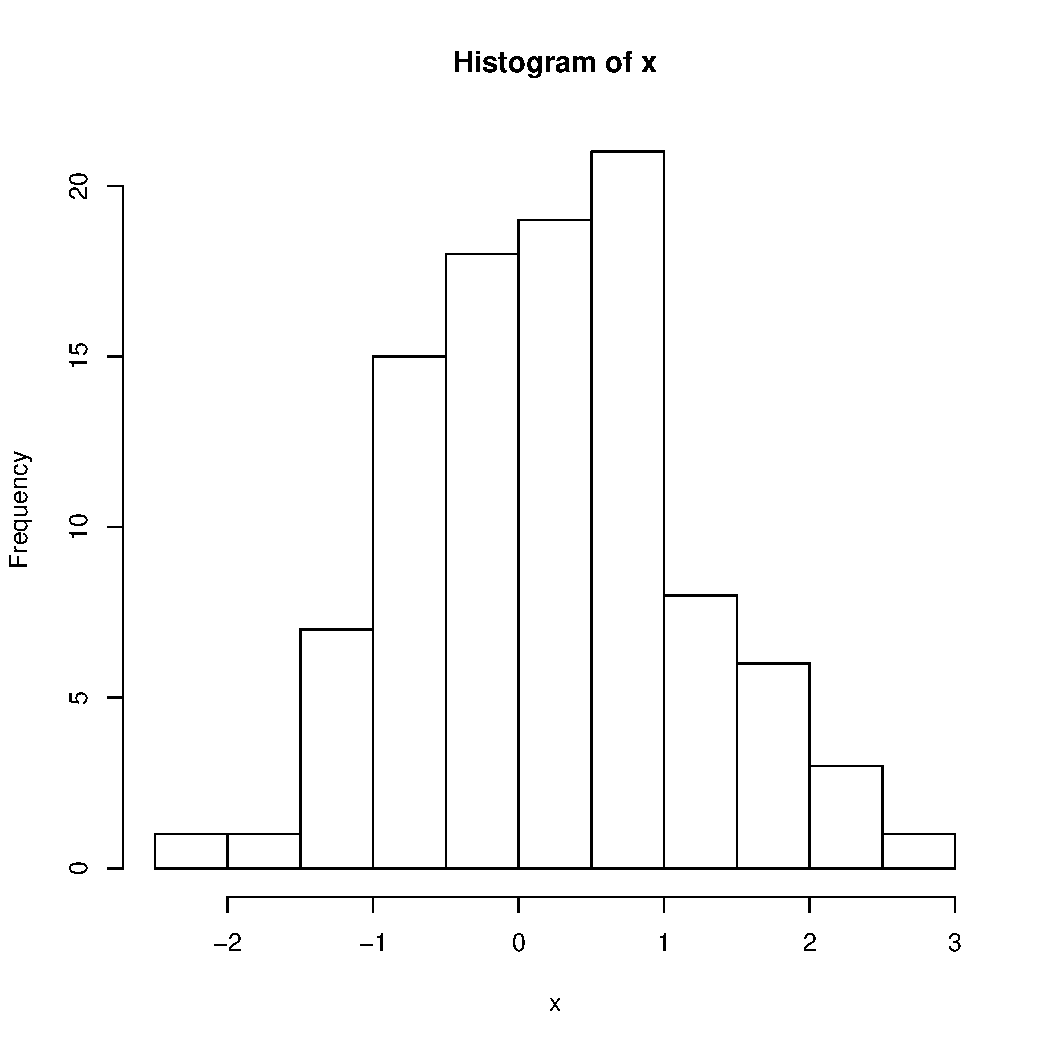
\includegraphics[width=\maxwidth]{figure/unnamed-chunk-8-1} 

\end{knitrout}

Looks vaguely normalish, no? [Of course, you can see that I'm drawing variates from the normal distribution, so this isn't surprising. Pretend you didn't see that part!] So what if we wanted to estimate the mean and var of the normal distribution that may have generated this set of draws.

How do we do this? The key statistical technique is to consider the likelihood.
Let's start by writing a function that computes the likelihood for "x" in a normal with unknown mean and var (collectively, "pars").

\begin{knitrout}
\definecolor{shadecolor}{rgb}{0.969, 0.969, 0.969}\color{fgcolor}\begin{kframe}
\begin{alltt}
\hlstd{likelihood}\hlkwb{<-}\hlkwa{function}\hlstd{(}\hlkwc{pars}\hlstd{,}\hlkwc{x}\hlstd{) \{} \hlcom{#see the first eqn here, http://mathworld.wolfram.com/NormalDistribution.html}
    \hlstd{tmp}\hlkwb{<-}\hlkwd{exp}\hlstd{(}\hlopt{-}\hlstd{(x}\hlopt{-}\hlstd{pars[}\hlnum{1}\hlstd{])}\hlopt{^}\hlnum{2}\hlopt{/}\hlstd{(}\hlnum{2}\hlopt{*}\hlstd{pars[}\hlnum{2}\hlstd{]))}
    \hlstd{tmp}\hlopt{/}\hlkwd{sqrt}\hlstd{(}\hlnum{2}\hlopt{*}\hlstd{pars[}\hlnum{2}\hlstd{]}\hlopt{*}\hlstd{pi)}
\hlstd{\}}
\end{alltt}
\end{kframe}
\end{knitrout}

To completely evaluate this function, we would need to know x and pars. We only know x (this is the problem of estimation in general: what are the values in pars?).
With known x, we can think of the likelihood as the "probability" of observing the draws x from a normal distribution with parameters pars.
That is, we are thinking of the likelihood as a function of pars (x is known).

Let's think about what we get if the mean is unknown and the SD=1
Q. what do you notice? 

\begin{knitrout}
\definecolor{shadecolor}{rgb}{0.969, 0.969, 0.969}\color{fgcolor}\begin{kframe}
\begin{alltt}
\hlstd{out}\hlkwb{<-}\hlkwd{list}\hlstd{()}
\hlkwa{for} \hlstd{(m} \hlkwa{in} \hlkwd{seq}\hlstd{(}\hlopt{-}\hlnum{1}\hlstd{,}\hlnum{1}\hlstd{,}\hlkwc{length.out}\hlstd{=}\hlnum{100}\hlstd{)) \{}
    \hlstd{like}\hlkwb{<-}\hlkwd{rep}\hlstd{(}\hlnum{NA}\hlstd{,}\hlkwd{length}\hlstd{(x))}
    \hlkwa{for} \hlstd{(i} \hlkwa{in} \hlnum{1}\hlopt{:}\hlkwd{length}\hlstd{(x)) \{}
        \hlstd{like[i]}\hlkwb{<-}\hlkwd{likelihood}\hlstd{(}\hlkwd{c}\hlstd{(m,}\hlnum{1}\hlstd{),x[i])}
    \hlstd{\}}
    \hlkwd{c}\hlstd{(}\hlkwd{c}\hlstd{(m,}\hlkwd{prod}\hlstd{(like)))}\hlkwb{->}\hlstd{out[[}\hlkwd{as.character}\hlstd{(m) ]]}
\hlstd{\}}
\hlkwd{plot}\hlstd{(}\hlkwd{do.call}\hlstd{(}\hlstr{"rbind"}\hlstd{,out),}\hlkwc{type}\hlstd{=}\hlstr{"b"}\hlstd{)} \hlcom{#this is a likelihood surface where we're seeing the likelihood as a function of the unknown mean}
\end{alltt}
\end{kframe}
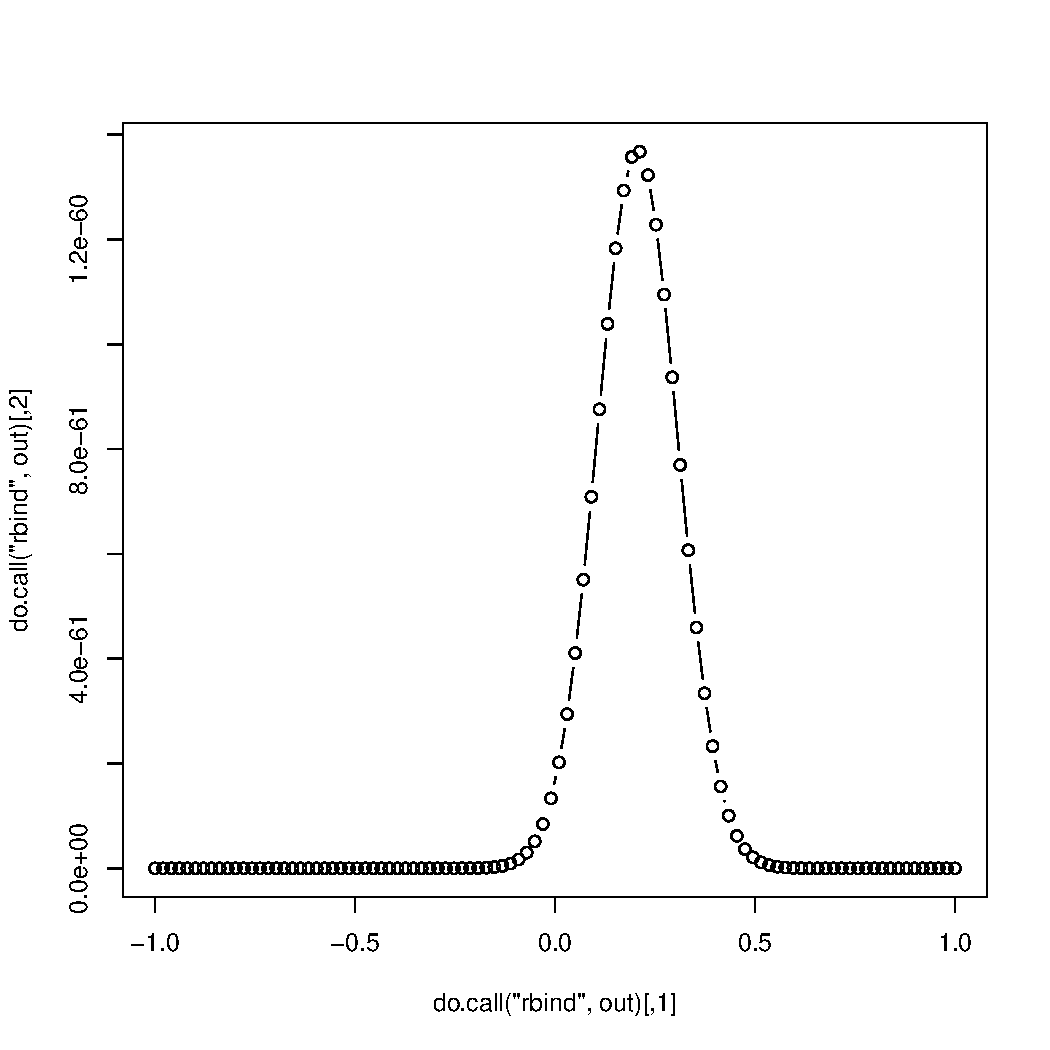
\includegraphics[width=\maxwidth]{figure/unnamed-chunk-10-1} 

\end{knitrout}


From a computational perspective, working with the products of small numbers is very unstable. So we instead work with the sum of the logs.
Why is this ok? First of all, $log(xy)=log(x) + log(y)$
Second, log(f(x)) is a monotic transformation of f(x). So if we maximize log(f(x)) funtion, then we've also maximized f(x)
Below is a function that will do this.

Q. How do our estimates vary in accuracy as a function of the sample size (change 100 to something much bigger and much smaller in the top line)

\begin{knitrout}
\definecolor{shadecolor}{rgb}{0.969, 0.969, 0.969}\color{fgcolor}\begin{kframe}
\begin{alltt}
\hlstd{ll}\hlkwb{<-}\hlkwa{function}\hlstd{(}\hlkwc{pars}\hlstd{,}\hlkwc{x}\hlstd{) \{}
    \hlstd{likelihood}\hlkwb{<-}\hlkwa{function}\hlstd{(}\hlkwc{pars}\hlstd{,}\hlkwc{x}\hlstd{) \{}
        \hlstd{tmp}\hlkwb{<-}\hlkwd{exp}\hlstd{(}\hlopt{-}\hlstd{(x}\hlopt{-}\hlstd{pars[}\hlnum{1}\hlstd{])}\hlopt{^}\hlnum{2}\hlopt{/}\hlstd{(}\hlnum{2}\hlopt{*}\hlstd{pars[}\hlnum{2}\hlstd{]))}
        \hlstd{tmp}\hlopt{/}\hlkwd{sqrt}\hlstd{(}\hlnum{2}\hlopt{*}\hlstd{pars[}\hlnum{2}\hlstd{]}\hlopt{*}\hlstd{pi)}
    \hlstd{\}}
    \hlstd{like}\hlkwb{<-}\hlkwd{rep}\hlstd{(}\hlnum{NA}\hlstd{,}\hlkwd{length}\hlstd{(x))}
    \hlkwa{for} \hlstd{(i} \hlkwa{in} \hlnum{1}\hlopt{:}\hlkwd{length}\hlstd{(x)) \{}
        \hlstd{like[i]}\hlkwb{<-}\hlkwd{likelihood}\hlstd{(pars,x[i])}
    \hlstd{\}}
    \hlopt{-}\hlnum{1}\hlopt{*}\hlkwd{sum}\hlstd{(}\hlkwd{log}\hlstd{(like))}
\hlstd{\}}
\hlkwd{optim}\hlstd{(}\hlkwc{par}\hlstd{=}\hlkwd{c}\hlstd{(}\hlopt{-}\hlnum{2}\hlstd{,}\hlnum{2}\hlstd{),ll,}\hlkwc{x}\hlstd{=x)}\hlopt{$}\hlstd{par} \hlcom{#these are the mean and variance estimates produced by maximum likelihood.}
\end{alltt}
\begin{verbatim}
## [1] 0.2058405 0.9189130
\end{verbatim}
\end{kframe}
\end{knitrout}


\section{Item Quality}

Consider the item statistics (p-values \& item-total correlations) discussed in the Crocker \& Algina text. What do you think? As a point of contrast, consider them vis-a-vis the item statistics generated by this data:

\begin{knitrout}
\definecolor{shadecolor}{rgb}{0.969, 0.969, 0.969}\color{fgcolor}\begin{kframe}
\begin{alltt}
\hlstd{emp_rash} \hlkwb{<-} \hlkwd{read.table}\hlstd{(}\hlstr{"emp-rasch.txt"}\hlstd{)}
\hlstd{rasch} \hlkwb{<-} \hlkwd{read.table}\hlstd{(}\hlstr{"rasch.txt"}\hlstd{)}
\end{alltt}
\end{kframe}
\end{knitrout}


\section{Buffon's Needle Problem}

\end{document}
